\chapter{Introducción}
\label{cap:introduccion}

\section{Robótica móvil}
\label{cap:roboticamovil}
Los robots móviles son máquinas con la capacidad de desplazarse por un entorno. Para ello hacen uso de un sistema de automoción, ya sean ruedas, patas u orugas. 
La robótica móvil está sufriendo un gran crecimiento debido al abaratamiento del hardware y las grandes oportunidades que nos ofrecen, tanto en materia de educación como en materia industrial. 
Cuando nos encontramos con un problema en el que un robot móvil puede ser la mejor solución tendremos que tener en cuenta los siguientes problemas a solucionar:
\begin{itemize}
\item \textbf{Percepción} Para resolver este problema equiparemos a nuestro robot de sensores, como puede ser una cámara, un láser, sensores de odometría o bumpers para obtener información acerca de qué hay en el escenario en el que se encuentra el robot.
\item \textbf{Localización} Una vez resuelto el problema de conocer que hay cerca del robot, necesitamos conocer la posición del robot dentro del escenario. Esto se puede resolver con algoritmos como MonteCarlo, con cámaras cenitales, triangulación con balizas, etc. Para resolver la localización también es común el uso de mapas. 
\item \textbf{Navegación} La característica principal de los robots móviles es que tienen la capacidad de desplazarse, pero la navegación no solo se cumple cuando el robot se mueve, el robot debe moverse a un punto determinado, de una forma segura, es decir sin chocar con los objetos del escenario, y de la forma más eficaz posible. Dentro de la navegación se pueden distinguir 2 partes, la navegación local que se ocupa del movimiento del robot y de evitar obstáculos y la navegación global qué establece rutas.
\item \textbf{Inteligencia} El siguiente problema se encuentra en un nivel de abstracción más alto. El problema de la inteligencia se refiere a qué tiene que hacer el robot, qué finalidad debe cumplir.
\item \textbf{Autonomía} Habrá momentos en los que el robot deberá tomar algunas decisiones, en referencia a su estado en el escenario, por ejemplo si se acerca mucho a una pared, o si llega a su destino correctamente.
\item \textbf{Interacción con los humanos} Los robots suelen crearse para facilitarnos una tarea o asistirnos en nuestro día a día, por esto los robots deben contar con una interfaz hombre-maquina con la que comunicarnos cosas o con la que nosotros podamos ayudar al robot para así mejorar sus acciones.
\end{itemize}

\section{Mapeado}
\label{cap:mapeado}
Crear un mapa de un escenario puede sernos realmente útil ya que servirán al robot como fuente de información para resolver problemas de Localización y de Navegación. Estos mapas pueden ser creados por un humano, midiendo las paredes y los objetos de un escenario para más tarde transformarlo en una imagen que el robot pueda leer, o puede ser creado directamente con un robot móvil. Esta segunda opción nos permite realizar mapas de zonas que pueden resultar inaccesibles para el ser humano, como puede ser una zona radioactiva u otro planeta del sistema solar.

\begin{figure}[hbtp]
  \begin{center}
    \subfigure[Mapa láser]{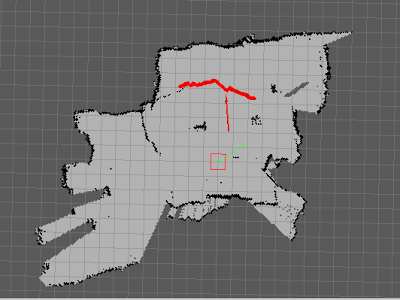
\includegraphics[width=6cm,height=5cm]{img/cap1/mapa1}}
    \subfigure[Mapa RGBD]{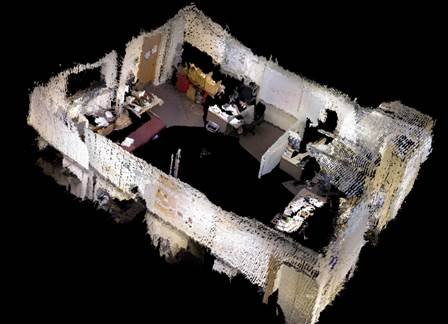
\includegraphics[width=6cm,height=5cm]{img/cap1/mapa2}}
  \end{center}
  \caption{Ejemplos de mapas}
  \label{fig:maps-ej}
\end{figure}
Para llevar a cabo el mapeo de un escenario con un robot móvil deberemos equipar a nuestro robot con sensores capaces de medir distancias, tales como una cámara RGBD o un láser. La cámara RGBD nos proporciona una nube de puntos en 3D, por lo que nos proporciona una información muy rica del entorno pero el tratamiento de esta información resulta muy costoso. El láser nos proporciona un array de distancias en 270º, estas distancias suelen ser muy precisas y su tratamiento es muy liviano, aunque solo contamos con el plano en el que se ubica el láser. 




\section{RoboCup@Home}
\label{cap:robocup}

\section{Estructura de la memoria}
\label{cap:estructuradelamemoria}


